\documentclass{article}

\usepackage[preprint]{neurips_2023}

\usepackage[utf8]{inputenc} % allow utf-8 input
\usepackage[T1]{fontenc}    % use 8-bit T1 fonts
\usepackage{hyperref}       % hyperlinks
\usepackage{url}            % simple URL typesetting
\usepackage{booktabs}       % professional-quality tables
\usepackage{amsfonts}       % blackboard math symbols
\usepackage{subcaption}
\usepackage{enumitem}
\usepackage{nicefrac}       % compact symbols for 1/2, etc.
\usepackage{microtype}      % microtypography
\usepackage{xcolor}         % colors
% \usepackage[colorlinks]{hyperref}
\usepackage[nameinlink,noabbrev]{cleveref}
\crefformat{figure}{\textsuperscript{#2#1#3}}
\crefformat{table}{\textsuperscript{#2#1#3}}
\usepackage{titlesec}
\usepackage{float}

\setcounter{secnumdepth}{4}

\titleformat{\paragraph}
{\normalfont\normalsize\bfseries}{\theparagraph}{1em}{}
\titlespacing*{\paragraph}
{0pt}{3.25ex plus 1ex minus .2ex}{1.5ex plus .2ex}


\title{An Exploration of Basic Methods for Handwritten Digit Classification}

\author{
	Brandon Szeto \thanks{160 lbs} \\
	Jacobs School of Engineering \\
	University of California, San Diego \\
	San Diego, CA 92122 \\
	\texttt{bszeto@ucsd.edu} \\
	\AND
	Darren Yu \thanks{130 lbs} \\
	Jacobs School of Engineering \\
	University of California, San Diego \\
	San Diego, CA 92122 \\
	\texttt{damiyu@ucsd.edu} \\
	\AND
	Nathaniel Thomas \thanks{200 lbs} \\
	Jacobs School of Engineering \\
	University of California, San Diego \\
	San Diego, CA 92122 \\
	\texttt{nathomas@ucsd.edu} \\
}

\begin{document}

\maketitle

\begin{figure}[H]
	\centering
	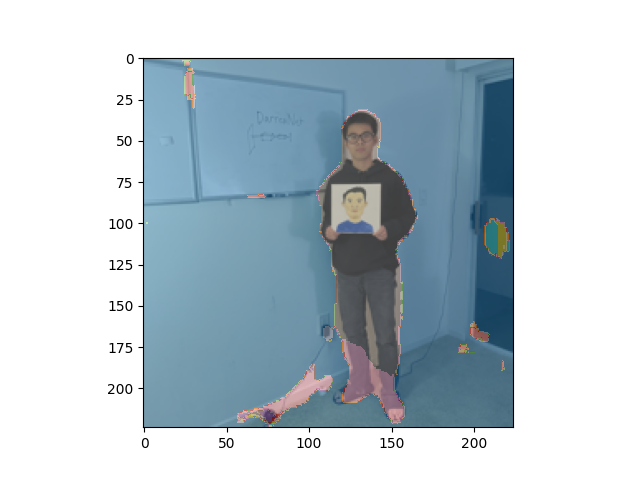
\includegraphics[width=0.5\textwidth]{plots/darren_inference}
	\caption{DarrenNet computing inference on Darren}
	\label{fig:inference}
\end{figure}

\begin{abstract}
	This abstract provides a succinct overview of our work focused on semantic segmentation using the PASCAL VOC-2007 dataset. Our approach involves leveraging a novel deep learning architecture tailored for semantic segmentation tasks. We meticulously preprocess the dataset, addressing challenges such as class imbalance and data augmentation to enhance model generalization. Through experimentation, we explore hyperparameter tuning strategies to optimize performance. Our results showcase a notable improvement in both percent correct and Mean Intersection over Union (IoU) metrics, underscoring the efficacy of our methodology. Additionally, we uncover intriguing insights into the model's behavior, shedding light on its strengths and potential areas for refinement. This work showcases a framework for accurate and nuanced semantic segmentation.
\end{abstract}


\section*{Introduction}

Semantic segmentation is the task of assigning each pixel in an image a specified label. A single image can be partitioned into multiple meaningful segments corresponding to a given object or region of interest. Labels are assigned to individual pixels, marking boundaries and shapes. Altogether, this task has many applications in computer vision including but not limited to autonomous driving, video surveillance, and object recognition.

In recent years, convolutional neural networks (CNNs) have proven to be an effective approach to semantic segmentation. Such models learn hierarchical features by capturing information using convolutional blocks. Convolutions and related techniques such as weight initialization, batch normalization, and pooling help avoid the flat, dense layers of a traditional fully connected neural network allowing for less computation and improved feature maps.

\subsection*{Xavier Weight Initialization}
In our architecture, we use Xavier weight initialization. In Uniform Xavier Initialization, a layer’s weights are chosen from a random uniform distribution bounded between

\begin{equation}
	\pm \displaystyle\frac{\sqrt{6}}{\sqrt{n_i + n_{i + 1}}}
\end{equation}

where $n_i$ is the number of incoming network connections and $n_{i + 1}$ is the number of outgoing network connections.

In Normal Xavier Initialization, a layer’s weights are chosen from a normal distribution with

\begin{equation}
	\sigma = \displaystyle\frac{\sqrt{2}}{\sqrt{n_i + n_{i + 1}}}
\end{equation}

where $n_i$ is the number of incoming network connections and $n_{i + 1}$ is the number of outgoing network connections.

The Xavier initialization was created in response to the problem of vanishing and exploding gradients in deep neural networks in the context of symmetric nonlinearities (sigmoid, tanh). The intuition is that the weights should not be intialized randomly, but rather proportional to the size of two connected layers. As a result, the variance of activations and gradients would be maintained through the layers of a deep network.

\subsection*{Kaiming Weight Initialization}
With the rise of ReLU, the nonlinearity can no longer be assumed to be symmetric. As such, the assumptions made by the Xavier Weight Initialization fall apart. In 2015, He et. al demonstrated that a ReLU layer typically has a standard deviation close to

\begin{equation}
	\sqrt{\displaystyle\frac{n_{i}}{2}}
\end{equation}

where $n_i$ is the number of incoming network connections. As such, weights initially chosen from a normal distribution should be weighted by $\sqrt{\frac{n_{i}}{2}}$, with bias tensors initalized to zero.

\subsection*{Batch Normalization}
During the training of a neural network, at each layer, inputs (activations) change as the parameters of the previous layers get updated. Batch normalization normalizes the activations of each layer by subtracting the mean and dividing by the standard deviation of the activations within a mini-batch. We implement batch normalization using PyTorch's \texttt{nn} module implementation. For example, we define a layer used for batch normalization as

\begin{center}
\texttt{self.bnd1 = nn.BatchNorm2d(32)}
\end{center} 

This ensures that the inputs to each layer have a consistent distribution, which helps in stabilizing the training process.


\section*{Related Works}

\subsection*{U-Net} 
U-Net \cite{unet} has proven to be highly effective for biomedical image segmentation tasks. Its architecture features a contracting path to capture context and an expansive path for precise localization. The innovative use of skip connections facilitates the flow of fine-grained details across different layers, enhancing the model's ability to accurately delineate object boundaries.

% \subsection*{ERFNet} 
% ERFNet \cite{erfnet} introduces a novel factorized convolutional layer that significantly reduces the number of parameters while maintaining expressive power. This reduction in parameters enables faster inference without compromising performance, making it well-suited for deployment in resource-constrained environments.

\subsection*{ResNet} 
ResNet \cite{resnet} addresses the challenges of training very deep neural networks by employing residual connections. These connections enable the direct flow of information across layers, mitigating the vanishing gradient problem and facilitating the training of extremely deep networks.

\subsection*{Relevance to our model} 
We test the performance of the above models on the image segmentation task using the PASCAL VOC-2007 dataset. We look for differences in the models and their relative performance in comparison to the basic fully connected network that we started with.

% The U-Net-inspired design prioritizes spatial precision and context awareness, crucial for tasks such as image segmentation, while the ResNet-inspired residual connections promote efficient training and enable the effective propagation of information through deep networks. (To add if we actually create a custom model)


\section*{Methods}
% In the Methods section, you should describe the implementation and architectural details of your system - in particular, this addresses how you approached the problem and the design of your solution. For those who believe in reproducible science, this should be fine-grained enough such that somebody could implement your model/algorithm and reproduce the results you claim to achieve.

\begin{figure}[H]
	\centering
	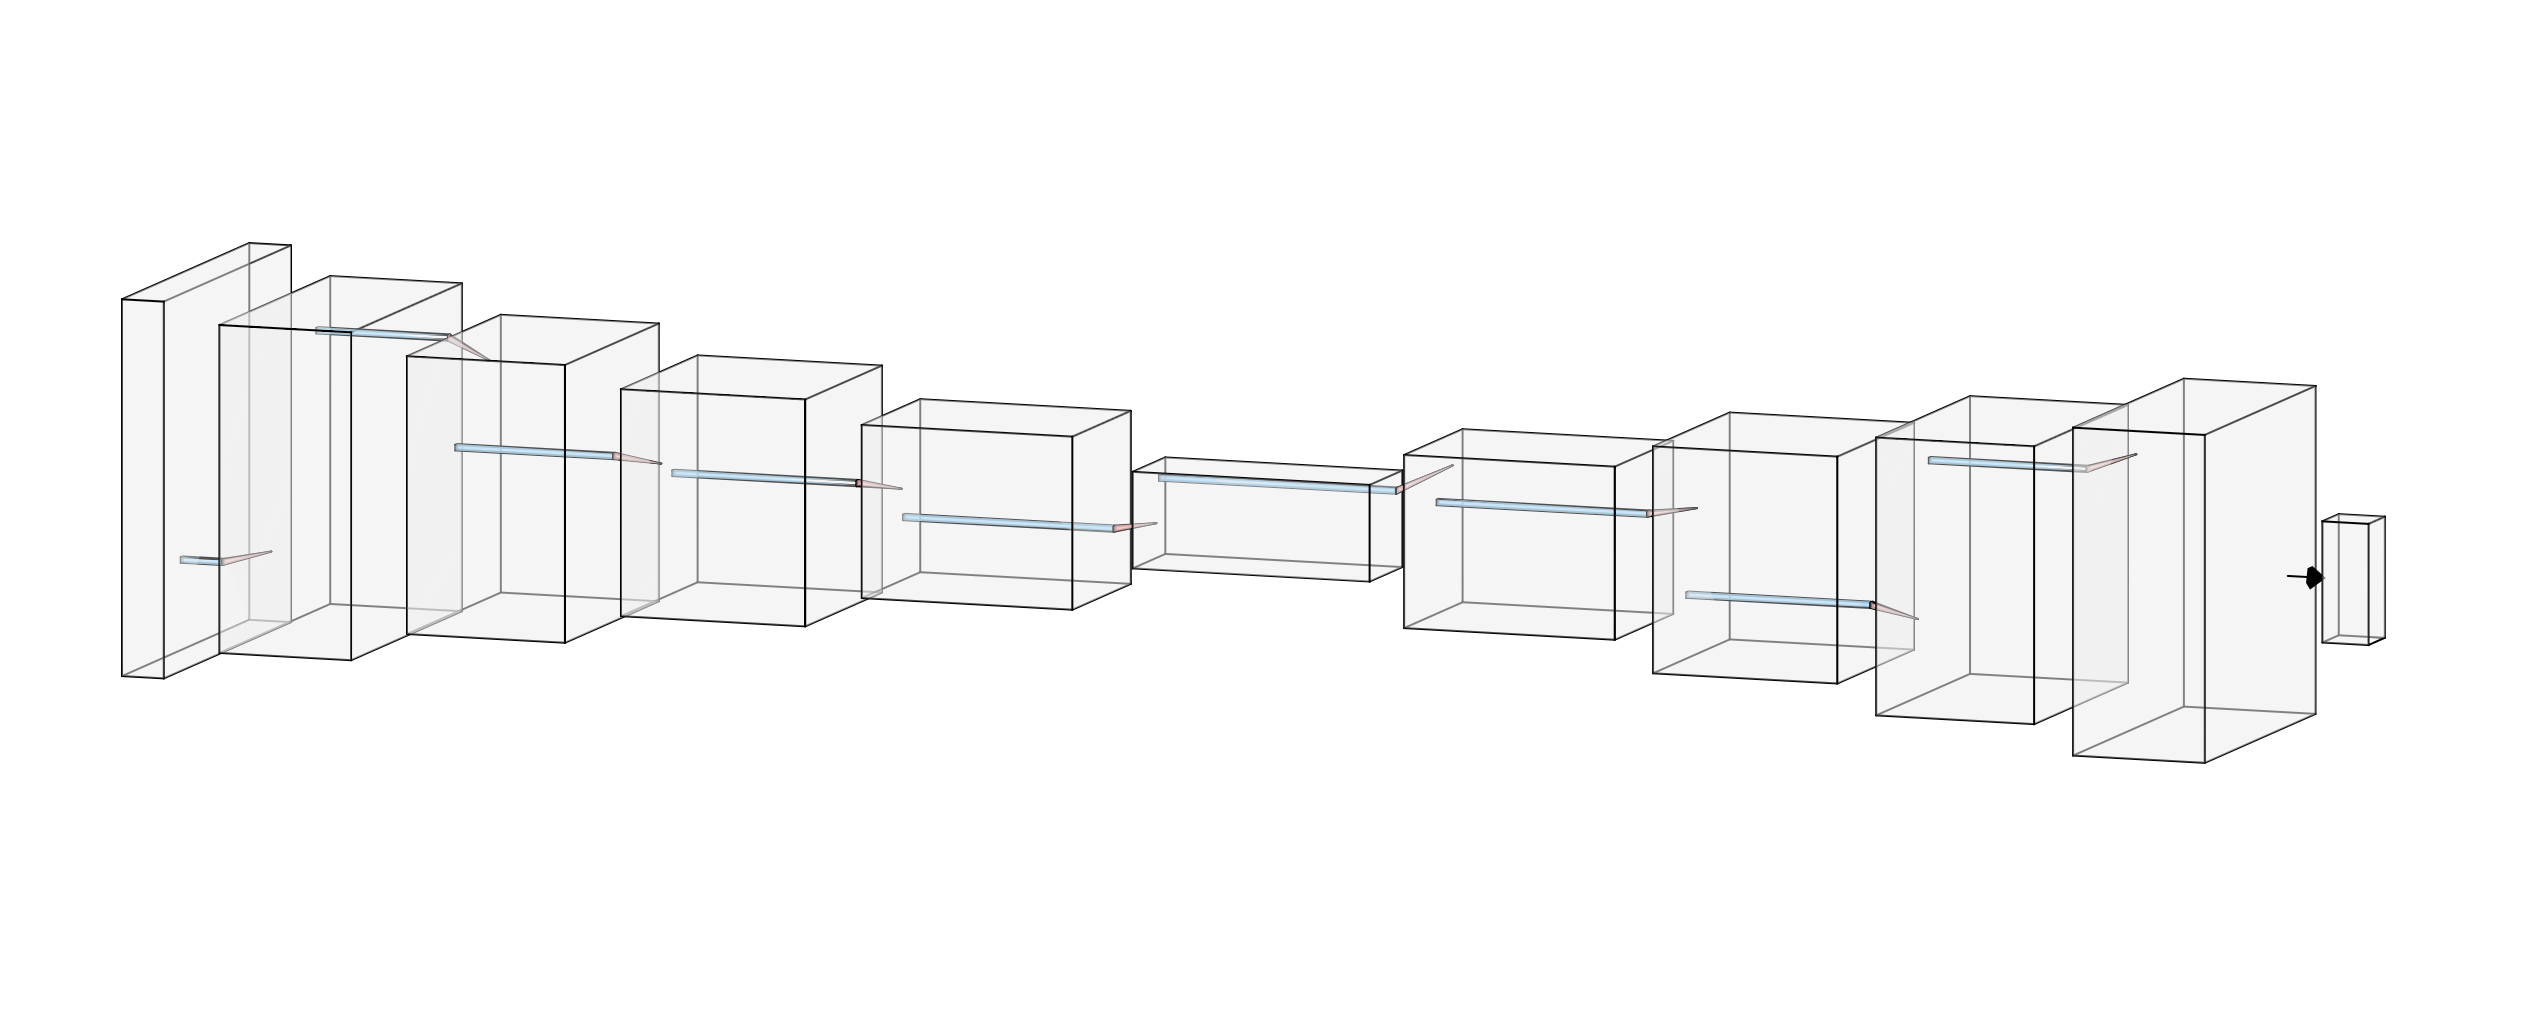
\includegraphics[width=\textwidth]{images/architecture}
	\caption{Visualization of System Architecture}
	\label{fig:architecture}
\end{figure}

\section*{Baseline}
% (a) Baseline (5 pt): You should describe the baseline architecture, stating the appropriate activation function on the last layer of the network, the loss criterion, weights initialization scheme and the gradient descent optimizer you used.
Our baseline architecture consists of an encoder, decoder, classifier, and activation. We used the Adam gradient descent optimizer

\subsubsection*{Encoder}
We have five convolutional layers that increases the depth of the orginal 3 channels to 32 to 64 to 128 to 256 to 512 each using a size 3 kernel, padding of 1, a stride of 2, and no dilation. Each layer sees a small decrease in the height and width of the layer according to the expression $\frac{W - F + 2P}{2} + 1$. The outputs of each convolutional layer are subsequently passed through a ReLU activation function and a batch normalization layer.

\subsubsection*{Decoder}
We have five deconvolutional, or upsampling layers that decreases the depth of the final 512 deep layer output from the encoder. This is decreases from 512 to 256 to 128 to 64 to 32 each using a size 3 kernel, padding of 1, a stride of 2, and no dilation. Each layer sees a small decrease in the height and width of the layer according to the expression $S(W - 1) + F - 2P$. Similarly, the outputs of each deconvolutional layer are subsequently passed through a ReLU activation function and a batch normalization layer.

\subsubsection*{Classifier and Activation}
In our final layer, we have a $1 \times 1$ convolutional kernel working as a classifier, and a softmax activation layer.

\section*{Improvements Over Baseline}
% (b) Improvements over Baseline (5 pt): You should describe the approaches you took to improve over the baseline model.

\subsubsection*{Data Augmentation}
To enhance the robustness of our model, we applied data augmentation techniques to our dataset. This involved performing various transformations on the input images, such as mirror flips, rotations, and crops. During the process, we must ensure that the same transformations are applied to the corresponding labels to maintain data integrity throughout the augmentation process.

\subsubsection*{Cosine Annealing}
In order to optimize the learning rate dynamically throughout the training process, we implemented the cosine annealing learning rate scheduler. This technique adjusts the learning rate in a cosine-shaped manner, effectively annealing it towards zero as training progresses. By aligning the learning rate adjustments with the number of epochs, we aim to improve the convergence and generalization capabilities of our model.

\subsubsection*{Class Imbalance}
To mitigate the challenges posed by class imbalance, particularly addressing rare classes, we employed strategies to alleviate this issue. One approach is to apply a weighted loss criterion, which assigns higher weights to the infrequent classes during the optimization process. By doing so, we incentivize the network to pay more attention to these underrepresented classes, thus improving its ability to accurately classify them. Otherwise, the model could simply learn to label the entire image the background and still achieve decent pixel accuracy.

\section*{Experimentation}

% (c) Experimentation (10 pt): Describe your two experimental CNN architectures(parts 5.a and 5.b) and the U-Net, each in a table, which the first column indicate the particular layer of your network, and the other columns state the layer’s dimensions (e.g. in-channels, out-channels, kernel-size, padding/stride) and activation function/non-linearity. Describe any regularization techniques (e.g. data augmentation) you used, parameter initialization methods, gradient descent optimization, and how you addressed the class-imbalance problem .
Below are the descriptions (in table format) and regularization techniques used for each architecture.

\subsection*{DarrenNet Architecture}
\begin{table}[H]
	\centering
	\label{tab:darrenyu}
	\setlength{\abovecaptionskip}{10pt}
	\begin{tabular}{|c|c|c|c|c|c|c|}
		\hline
		\textbf{Layer}    & \textbf{In} & \textbf{Out} & \textbf{Padding} & \textbf{Kernel} & \textbf{Stride} & \textbf{Activation} \\ \hline
		Initial Block     &             & 16           & 0                & 3x3             & 1               & ReLU                \\ \hline
		Downsampler 1     & 16          & 64           & 0                & 3x3             & 2               & ReLU                \\ \hline
		Non-bottleneck 1  & 64          & 64           & 0                & 3x3             & 1               & ReLU                \\ \hline
		Non-bottleneck 2  & 64          & 64           & 0                & 3x3             & 1               & ReLU                \\ \hline
		Non-bottleneck 3  & 64          & 64           & 0                & 3x3             & 1               & ReLU                \\ \hline
		Non-bottleneck 4  & 64          & 64           & 0                & 3x3             & 1               & ReLU                \\ \hline
		Non-bottleneck 5  & 64          & 64           & 0                & 3x3             & 1               & ReLU                \\ \hline
		Downsampler 2     & 64          & 128          & 0                & 3x3             & 2               & ReLU                \\ \hline
		Non-bottleneck 6  & 128         & 128          & 0                & 3x3             & 1               & ReLU                \\ \hline
		Non-bottleneck 7  & 128         & 128          & 0                & 3x3             & 1               & ReLU                \\ \hline
		Non-bottleneck 8  & 128         & 128          & 0                & 3x3             & 1               & ReLU                \\ \hline
		Non-bottleneck 9  & 128         & 128          & 0                & 3x3             & 1               & ReLU                \\ \hline
		Non-bottleneck 10 & 128         & 128          & 0                & 3x3             & 1               & ReLU                \\ \hline
		Non-bottleneck 11 & 128         & 128          & 0                & 3x3             & 1               & ReLU                \\ \hline
		Non-bottleneck 12 & 128         & 128          & 0                & 3x3             & 1               & ReLU                \\ \hline
		Non-bottleneck 13 & 128         & 128          & 0                & 3x3             & 1               & ReLU                \\ \hline
		Upsampler 1       & 128         & 64           & 0                & 3x3             & 1               & ReLU                \\ \hline
		Non-bottleneck 14 & 64          & 64           & 0                & 3x3             & 1               & ReLU                \\ \hline
		Non-bottleneck 15 & 64          & 64           & 0                & 3x3             & 1               & ReLU                \\ \hline
		Upsampler 2       & 64          & 16           & 0                & 3x3             & 1               & ReLU                \\ \hline
		Non-bottleneck 16 & 16          & 16           & 0                & 3x3             & 1               & ReLU                \\ \hline
		Non-bottleneck 17 & 16          & 16           & 0                & 3x3             & 1               & ReLU                \\ \hline
		Output Conv       & 16          & 21           & 0                & 2x2             & 2               & -                   \\ \hline
	\end{tabular}
	\caption{DarrenNet Architecture}
\end{table}

\begin{table}[H]
	\setlength{\abovecaptionskip}{10pt}
	\centering
	\begin{tabular}{|l|c|c|c|c|c|c|}
		\hline
		\textbf{Layer Name} & \textbf{In}          & \textbf{Out}         & \textbf{Padding}      & \textbf{Kernel Size} & \textbf{Stride} & \textbf{Activation} \\
		\hline
		conv1          & $n_{\text{channel}}$ & $n_{\text{channel}}$ & (1, 0)                & 3x1               & 1               & ReLU                \\
		\hline
		conv2          & $n_{\text{channel}}$ & $n_{\text{channel}}$ & (0, 1)                & 1x3               & 1               & ReLU                \\
		\hline
		conv3          & $n_{\text{channel}}$ & $n_{\text{channel}}$ & (1$\times$dilated, 0) & 3x1               & 1               & ReLU                \\
		\hline
		conv4          & $n_{\text{channel}}$ & $n_{\text{channel}}$ & (0, 1$\times$dilated) & 1x3               & 1               & ReLU                \\
		\hline
		bn1                 &                      &                      &                       &                      &                 &                     \\
		\hline
		bn2                 &                      &                      &                       &                      &                 &                     \\
		\hline
		dropout             &                      &                      &                       &                      &                 & 2D                  \\
		\hline
	\end{tabular}
	\caption{Non-bottleneck (DarrenNet)}
\end{table}

\begin{table}[H]
	\setlength{\abovecaptionskip}{10pt}
	\centering
	\begin{tabular}{|l|c|c|c|c|c|c|}
		\hline
		\textbf{Layer Name} & \textbf{In}            & \textbf{Out}                                 & \textbf{Padding} & \textbf{Kernel Size} & \textbf{Stride} & \textbf{Activation} \\
		\hline
		conv                & $in_{\text{channel}}$  & $out_{\text{channel}} - in_{\text{channel}}$ & 1           & 3x3               & 2               &                    \\
		\hline
		pool                &                       &                                             &                 & 2x2               & 2               &                    \\
		\hline
		bn                  & $out_{\text{channel}}$ & $out_{\text{channel}}$                       &                 &                     &                &                    \\
		\hline
	\end{tabular}
	\caption{DownsamplerBlock (DarrenNet)}
\end{table}

\begin{table}[H]
	\setlength{\abovecaptionskip}{10pt}
	\centering
	\begin{tabular}{|l|c|c|c|c|c|c|}
		\hline
		\textbf{Layer Name} & \textbf{In}            & \textbf{Out}           & \textbf{Padding} & \textbf{Kernel Size} & \textbf{Stride} & \textbf{Activation} \\
		\hline
		conv                & $in_{\text{channel}}$  & $out_{\text{channel}}$ & (1, 1)           & 3x3               & 2               &                    \\
		\hline
		bn                  & $out_{\text{channel}}$ & $out_{\text{channel}}$ &                 &                     &                &                    \\
		\hline
	\end{tabular}
	\caption{UpsamplerBlock (DarrenNet)}
\end{table}

\subsection*{DarrenNet Techniques}
In our DarrenNet architecture, we use horizontal and vertical flipping, Kaiming weight initialization, cosine annealing, and add extra penalty to loss inversely proportional to the frequency of a given class pixel.

\subsection*{Transfer Learning Architecture}
\begin{table}[H]
	\centering
	\label{tab:transfer}
	\setlength{\abovecaptionskip}{10pt}
	\begin{tabular}{|c|c|c|c|c|c|c|}
		\hline
		\textbf{Layer} & \textbf{In} & \textbf{Out} & \textbf{Padding} & \textbf{Kernel} & \textbf{Stride} & \textbf{Activation} \\ \hline
		encoder          &            &            &                 &              &                &                 \\ \hline
		deconv1        & 512         & 256           & 1                & 3x3             & 2               & ReLU                \\ \hline
		deconv1        & 512         & 256           & 1                & 3x3             & 2               & ReLU                \\ \hline
		deconv2        & 256         & 128           & 1                & 3x3             & 2               & ReLU                \\ \hline
		deconv3        & 128         & 64           & 1                & 3x3             & 2               & ReLU                \\ \hline
		deconv4        & 64         & 32           & 1                & 3x3             & 2               & ReLU                \\ \hline
		conv        & 32         & 21           & 1                & 3x3             & 2               & Softmax                \\ \hline
	\end{tabular}
	\caption{Transfered Encoder to Basic FCN Architecture}
\end{table}

\subsection*{Transfer Learning Techniques}
% In transfer learning, we use horizontal and vertical flipping, Kaiming weight initialization, cosine annealing, and add extra penalty to loss inversely proportional to the frequency of a given class pixel.

\subsection*{UNet Architecture}
\begin{table}[H]
	\centering
	\label{tab:unet}
	\setlength{\abovecaptionskip}{10pt}
	\begin{tabular}{|c|c|c|c|c|c|c|}
		\hline
		\textbf{Layer} & \textbf{In} & \textbf{Out} & \textbf{Padding} & \textbf{Kernel} & \textbf{Stride} & \textbf{Activation} \\ \hline
		conv1          & 3           & 64           & 1                & 3x3             & 1               & ReLU                \\ \hline
		conv2          & 64          & 64           & 1                & 3x3             & 1               & ReLU                \\ \hline
		pool1          & 64          & 64           & 0                & 2x2             & 2               &                     \\ \hline
		conv3          & 64          & 128          & 1                & 3x3             & 1               & ReLU                \\ \hline
		conv4          & 128         & 128          & 1                & 3x3             & 1               & ReLU                \\ \hline
		pool2          & 128         & 128          & 0                & 2x2             & 2               &                     \\ \hline
		conv5          & 128         & 256          & 1                & 3x3             & 1               & ReLU                \\ \hline
		conv6          & 256         & 256          & 1                & 3x3             & 1               & ReLU                \\ \hline
		pool3          & 256         & 256          & 0                & 2x2             & 2               &                     \\ \hline
		conv7          & 256         & 512          & 1                & 3x3             & 1               & ReLU                \\ \hline
		conv8          & 512         & 512          & 1                & 3x3             & 1               & ReLU                \\ \hline
		pool4          & 512         & 512          & 0                & 2x2             & 2               &                     \\ \hline
		conv9          & 512         & 1024         & 1                & 3x3             & 1               & ReLU                \\ \hline
		conv10         & 1024        & 1024         & 1                & 3x3             & 1               & ReLU                \\ \hline
		deconv1        & 1024        & 512          & 0                & 2x2             & 2               & ReLU                \\ \hline
		conv11         & 1024        & 512          & 1                & 3x3             & 1               & ReLU                \\ \hline
		conv12         & 512         & 512          & 1                & 3x3             & 1               & ReLU                \\ \hline
		deconv2        & 512         & 256          & 0                & 2x2             & 2               & ReLU                \\ \hline
		conv13         & 512         & 256          & 1                & 3x3             & 1               & ReLU                \\ \hline
		conv14         & 256         & 256          & 1                & 3x3             & 1               & ReLU                \\ \hline
		deconv3        & 256         & 128          & 0                & 2x2             & 2               & ReLU                \\ \hline
		conv15         & 256         & 128          & 1                & 3x3             & 1               & ReLU                \\ \hline
		conv16         & 128         & 128          & 1                & 3x3             & 1               & ReLU                \\ \hline
		deconv4        & 128         & 64           & 0                & 2x2             & 2               & ReLU                \\ \hline
		conv17         & 64          & 64           & 1                & 3x3             & 1               & ReLU                \\ \hline
		conv18         & 64          & 64           & 1                & 3x3             & 1               & ReLU                \\ \hline
		output         & 64          & 21           & 0                & 1x1             & 1               & ReLU                \\ \hline
	\end{tabular}
	\caption{UNet Architecture}
\end{table}

\subsection*{UNet Techniques}
% In the unet architecture, we use horizontal and vertical flipping, Kaiming weight initialization, cosine annealing, and add extra penalty to loss inversely proportional to the frequency of a given class pixel.



\section*{Results}

% In the Results section, you should demonstrate your baseline model’s performance, perfor- mances for each of the parts of Q4.b and Q4.c. You should include both of the performance metrics described in Evaluation metrics (see part 1 above in Implementation Instructions). Please organize these results into a series of concise tables. The formatting is your choice, as long as it is easily interpretable.
% For each architecture include:
% (a) A single plot showing both training and validation loss curves;
% (b) Validation set pixel accuracy and average IoU.
% (c) Visualizations of the segmented output for any one image in the test set along with the original image. Use the color coding mapping in the voc.py for this (Please refer to visualize.ipynb for help on plotting).

\subsection*{Baseline FCN}

Our baseline FCN resulted in a 0.06 IOU and a 75\% pixel accuracy on the test set.

\begin{figure}[H]
	\centering
	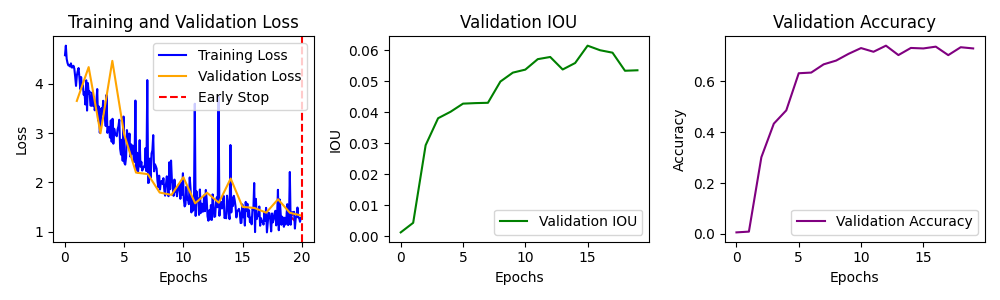
\includegraphics[width=\textwidth]{plots/baseline}
	\caption{Baseline Augmentation}
	\label{fig:baseline}
\end{figure}

\subsection*{FCN with augmentation}

Our FCN with augmentation resulted in a 0.06 IOU and a 72\% pixel accuracy on the test set. We noticed that the loss convergence
was slower.

\begin{figure}[H]
	\centering
	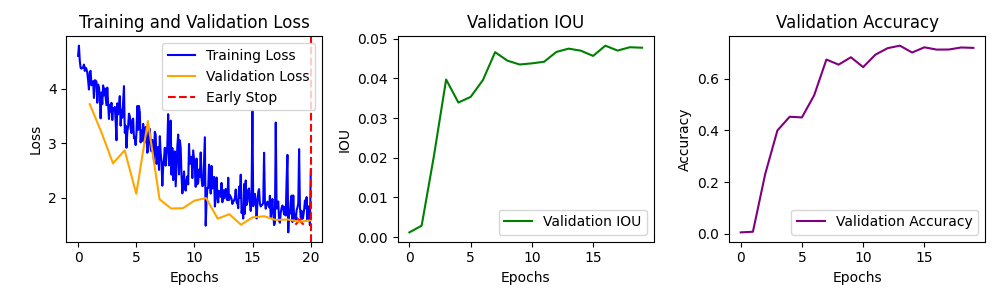
\includegraphics[width=\textwidth]{plots/baseline_augmentation}
	\caption{Baseline Augmentation}
	\label{fig:baseline_aug}
\end{figure}

\subsection*{FCN with Cosine Annealing LR}

Our FCN with Cosine Annealing LR resulted in a 0.05 IOU and a 74\% pixel accuracy on the test set.


\begin{figure}[H]
	\centering
	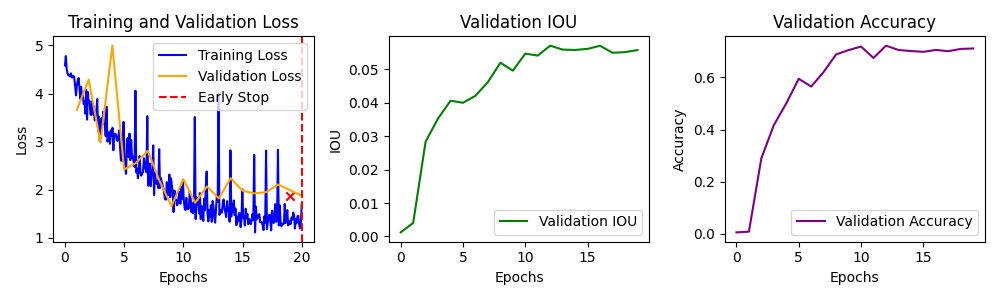
\includegraphics[width=\textwidth]{plots/baseline_cosine}
	\caption{Baseline Cosine}
	\label{fig:baseline_cos}
\end{figure}

\subsection*{FCN with Custom Class Weights}


Our FCN with custom class weights resulted in a slightly worse 0.04 IOU and a 67\% pixel accuracy on the test set.

\begin{figure}[H]
	\centering
	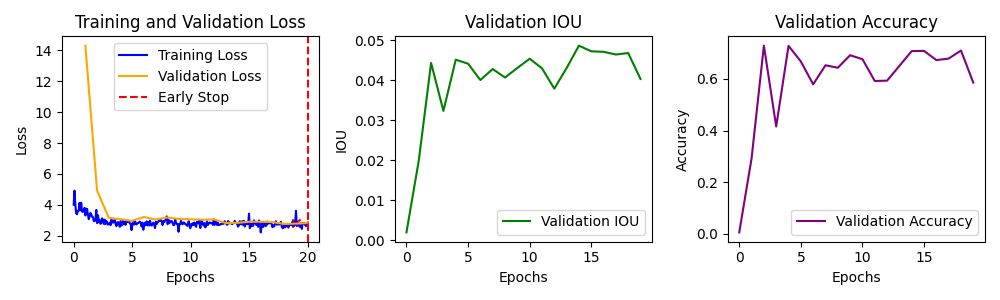
\includegraphics[width=\textwidth]{plots/baseline_weights}
	\caption{Baseline Weights}
	\label{fig:baseline_weights}
\end{figure}

\subsection*{DarrenNet}

In Figure \ref{fig:darren}, we observe the outcomes of DarrenNet. The model has a respectable IOU (0.05) and accuracy (75\%), while maintaining very fast training speeds.

\begin{figure}[H]
	\centering
	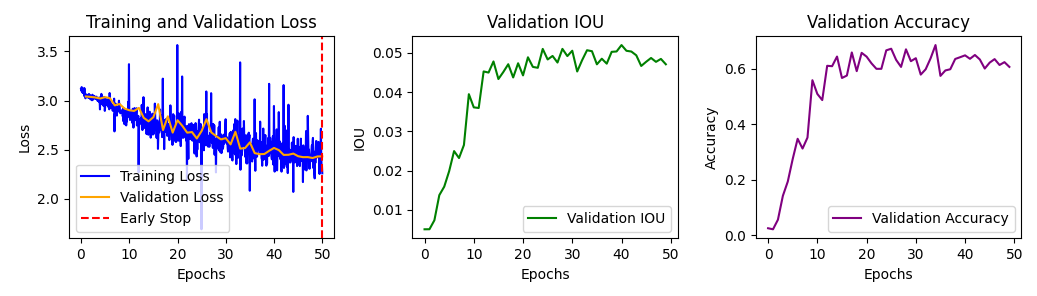
\includegraphics[width=\textwidth]{plots/darrennet}
	\caption{DarrenNet}
	\label{fig:darren}
\end{figure}


In Figure \ref{fig:darren_transfer}, we observe the outcomes of DarrenNet with transfer learning using resnet34's encoder. The model leverages pre-trained weights, demonstrating superior performance on the test set. The transfer learning strategy significantly boosts both IOU (0.10) and accuracy (78\%), indicating that the network effectively transfers knowledge from the source domain to the target domain.


\begin{figure}[H]
	\centering
	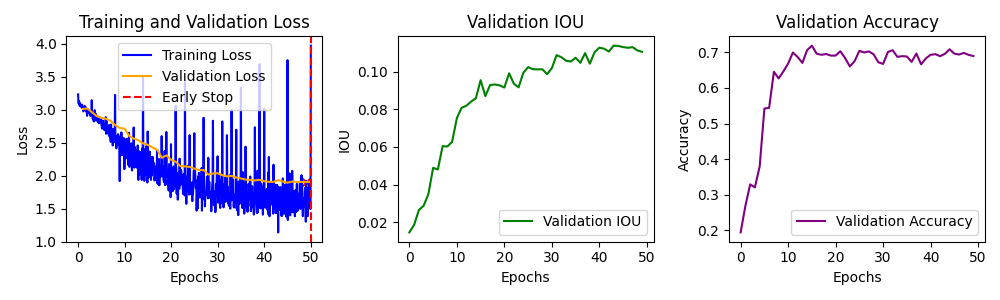
\includegraphics[width=\textwidth]{plots/darrennet_transfer}
	\caption{DarrenNet Transfer}
	\label{fig:darren_transfer}
\end{figure}


Figure \ref{fig:darren_transfer_aug} represents the results of DarrenNet with both transfer learning and data augmentation. This combination appears to be highly effective, as the model achieves impressive segmentation results on the test set. The incorporation of augmented data during training, along with knowledge transfer, contributes to enhanced generalization capabilities.

\begin{figure}[H]
	\centering
	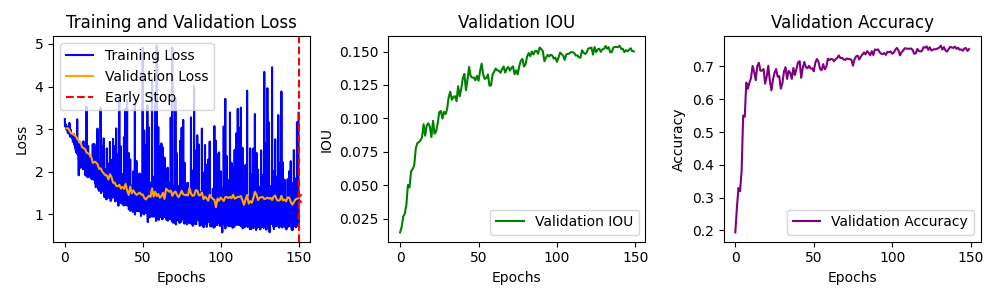
\includegraphics[width=\textwidth]{plots/darrennet_transfer_augment}
	\caption{DarrenNet Transfer Augment}
	\label{fig:darren_transfer_aug}
\end{figure}

Figure \ref{fig:darren_aug_aff} displays the results of the DarrenNet with Augment Affine and transfer learning. The model exhibits strong performance on the test set, achieving a high Intersection over Union (IOU) at 0.15 and 82\% accuracy. The augmentation techniques, particularly affine transformations, seem to enhance the model's ability to generalize well to unseen data, resulting in improved segmentation accuracy.

\begin{figure}[H]
	\centering
	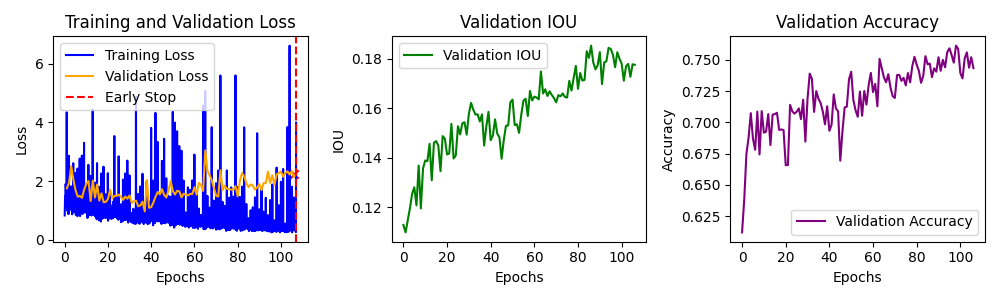
\includegraphics[width=\textwidth]{plots/darrennet_augment_affine}
	\caption{DarrenNet Augment Affine}
	\label{fig:darren_aug_aff}
\end{figure}


The UNet architecture's results are depicted in Figure \ref{fig:unet}. The model demonstrates below average segmentation performance, achieving poor IOU (0.05) and accuracy (0.55) on the test set.

\begin{figure}[H]
	\centering
	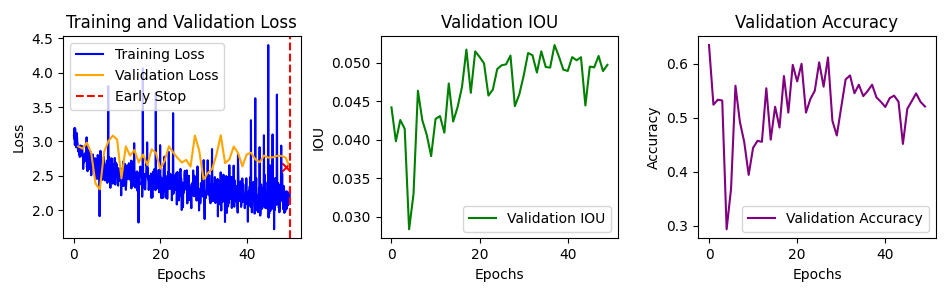
\includegraphics[width=\textwidth]{plots/unet}
	\caption{UNet}
	\label{fig:unet}
\end{figure}

In Figure \ref{fig:unet_transfer}, we observe the UNet with transfer learning. The model exhibits improved segmentation results compared to the non-transfer counterpart, showcasing the effectiveness of leveraging pre-trained weights. Transfer learning enhances the model's ability to understand and segment structures in the medical images, leading to higher IOU (0.08) and accuracy (79\%) on the test set.

\begin{figure}[H]
	\centering
	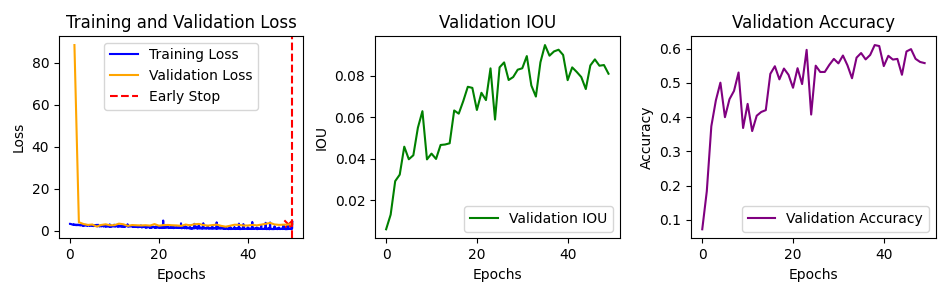
\includegraphics[width=\textwidth]{plots/unet_transfer}
	\caption{UNet Transfer}
	\label{fig:unet_transfer}
\end{figure}


We see the best results with DarrenNet that leverages pretrained ERFNet weights. Unet also
gives decent results, at least when it comes to detecting humans \ref{fig:comparison}.

\begin{figure}[H]
	\centering
	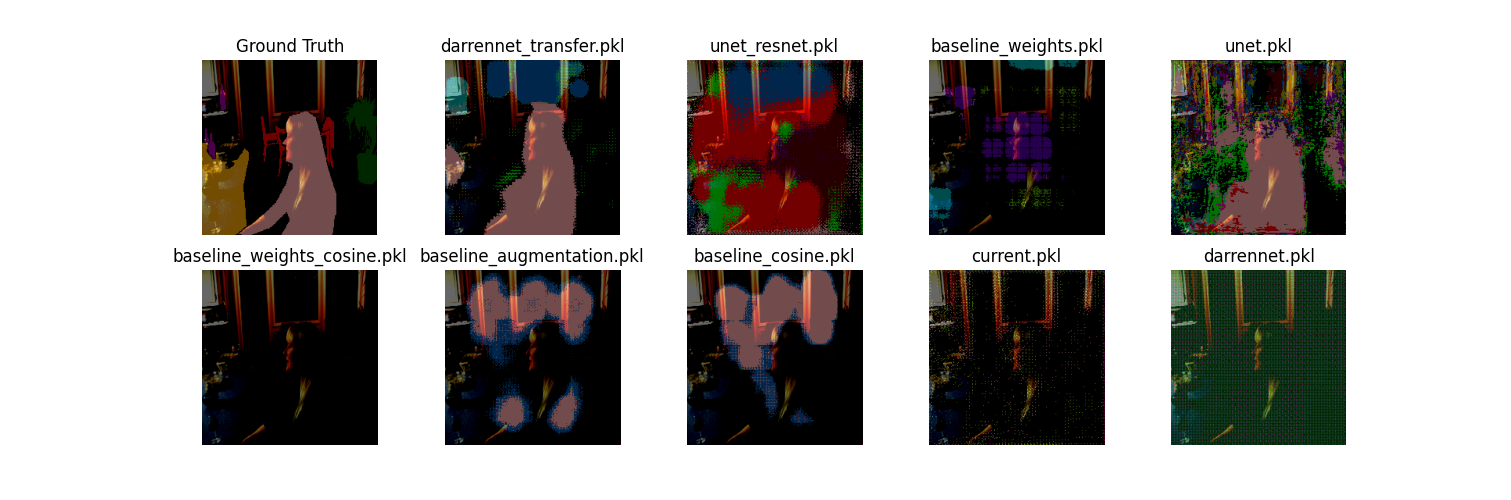
\includegraphics[width=\textwidth]{plots/comparison}
	\caption{Comparison between models}
	\label{fig:comparison}
\end{figure}


\section*{Discussion}
% The Discussion section should again have 3 sub-sections for Q3, Q4 and Q5. In each section you should discuss the benefits (and drawbacks if any) of the approaches/architectures you used and some discussion of why you think you got the results you got.
% Please discuss the following important points as well: How did the performance of your implementations differ? Discuss the performance differences with respect to the baseline (part 3), improved baseline (part 4) and compare the other implementations (part 5a, 5b, 5c) and mention them in their respective sub-sections. Also, draw insights from the plotted loss curves, tables and the visualizations.

\subsection*{Baseline}
The baseline model, though straightforward to implement, exhibited limitations in segmentation performance with an IOU of 0.06 and a pixel accuracy of 75%. The simplicity of the architecture hindered its ability to capture intricate features in the data.

\subsection*{Improved Baseline (FCN with Augmentation)}
In an effort to address overfitting, the baseline model was enhanced with data augmentation. Despite these improvements, the model faced challenges with slower loss convergence and only achieved a marginal increase in performance, resulting in an IOU of 0.06 and a decreased pixel accuracy of 72%.

\subsection*{DarrenNet:}
DarrenNet, incorporating advanced architectural features and augmentation techniques such as Affine transformations, displayed notable improvements with an IOU of 0.15 and a pixel accuracy of 82%. The architecture and augmentation strategy played pivotal roles in enhancing segmentation results.

\subsection*{Transfer Darrennet:}
The application of transfer learning with DarrenNet, utilizing pre-trained weights from resnet34, demonstrated significant performance gains with an IOU of 0.10 and a pixel accuracy of 78%. Successful knowledge transfer from the source domain contributed to the improved segmentation performance.

\subsection*{UNet:}
The UNet architecture, characterized by its ability to capture detailed spatial information, showed below-average baseline performance with an IOU of 0.05 and a pixel accuracy of 55%. However, when integrated with transfer learning, UNet outperformed the baseline, achieving an IOU of 0.08 and a pixel accuracy of 79%.

\subsection*{Performance Differences (Between Implementations):}
Comparative analysis revealed that DarrenNet consistently outperformed the baseline, showcasing the significance of architectural enhancements. Transfer learning, as evidenced in both Transfer DarrenNet and UNet with transfer, played a critical role in improving segmentation results, emphasizing the importance of leveraging pre-trained weights for feature extraction.

\subsection*{Insights from Loss Curves, Tables, Visualizations:}
Examination of loss convergence in the improved baseline highlighted challenges in augmentation effectiveness. Visualizations, loss curves, and performance metrics provided insights into the impact of architectural choices and transfer learning strategies, offering valuable information for further model refinement.


% Baseline:
% - Benefits
% - Drawbacks
% - Why we got the results we got
%
% Improved baseline:
% - Benefits
% - Drawbacks
% - Why we got the results we got
%
% DarrenNet:
% - Benefits
% - Drawbacks
% - Why we got the results we got
%
% Transfer Darrennet:
% - Benefits
% - Drawbacks
% - Why we got the results we got
%
% UNet:
% - Benefits
% - Drawbacks
% - Why we got the results we got
%
% Performance Differences (between implementations)
%
% Insights from loss curves, tables, visualizations


\section*{Contributions}

\textbf{Brandon Szeto}:

\textbf{Darren Yu}: Abstract, team name

\textbf{Nathaniel Thomas}:


\section*{References}

\medskip

{
	\small

	\begin{enumerate}[label={[\arabic*]}]
		\item \textit{Convnets}. (2024) University of California, San Diego, pp. 45-67.
	\end{enumerate}
}


% \input{sections/conclusion}

\end{document}
